\section{Simulation Analysis}
\label{sec:simulation} 

In these section we represent the plots that were produced by doing operating point using Ngspice. These plots represents the Voltage on Envelope Detector and the output voltage of the circuit.

\FloatBarrier
\begin{figure}
  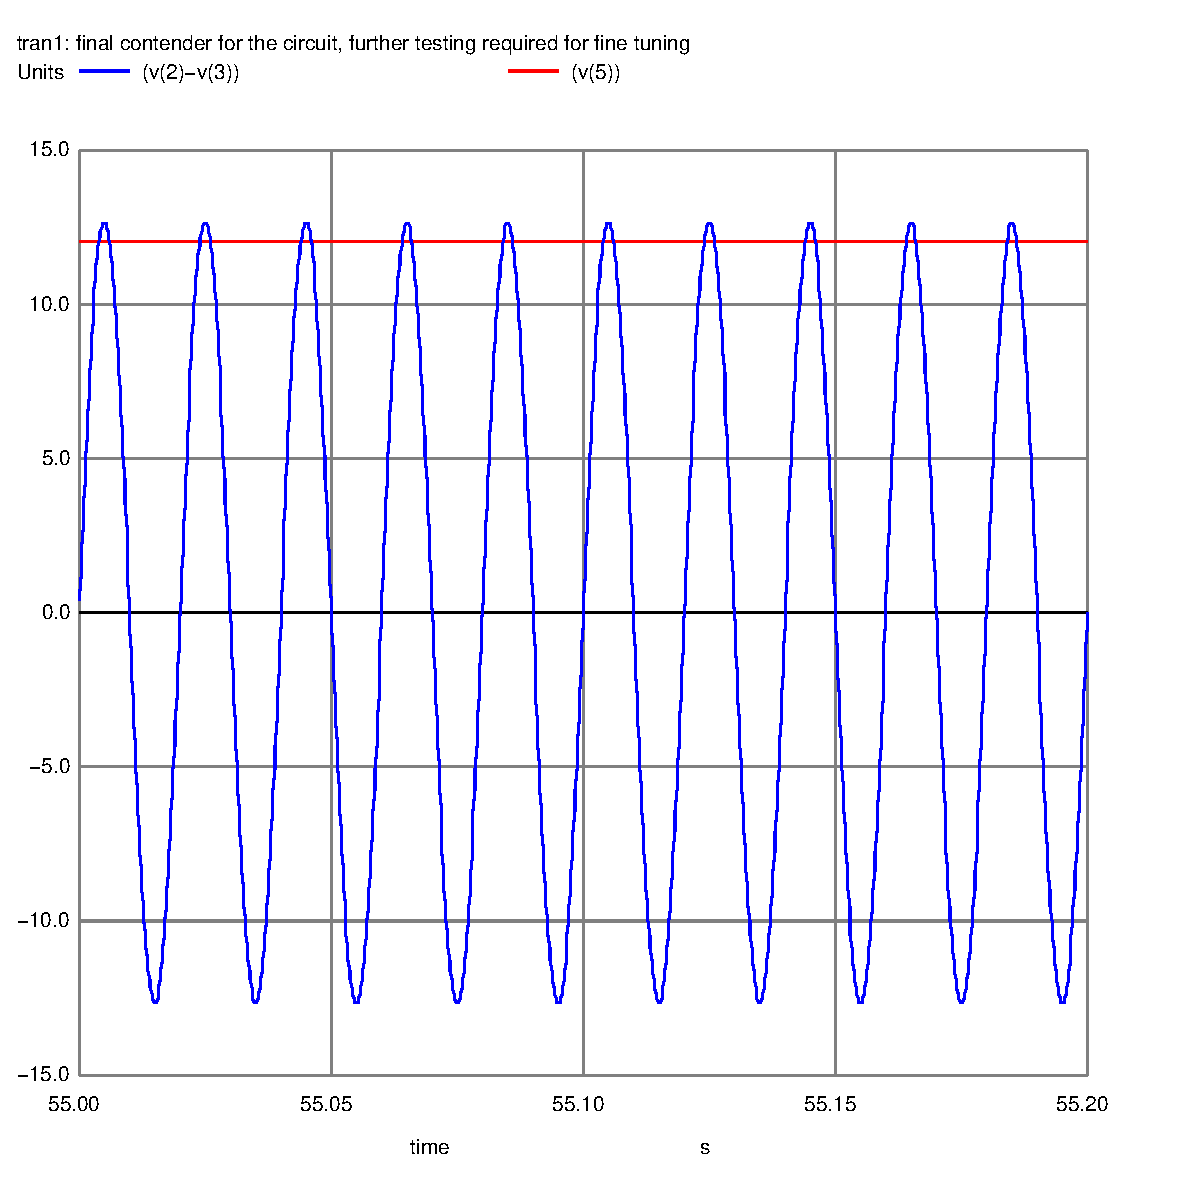
\includegraphics[width=\linewidth]{out.ps}
  \caption{Envelope Detector and Output Voltages}
  \label{fig:theoplots}
\end{figure}
\FloatBarrier 

\FloatBarrier
\begin{figure}
  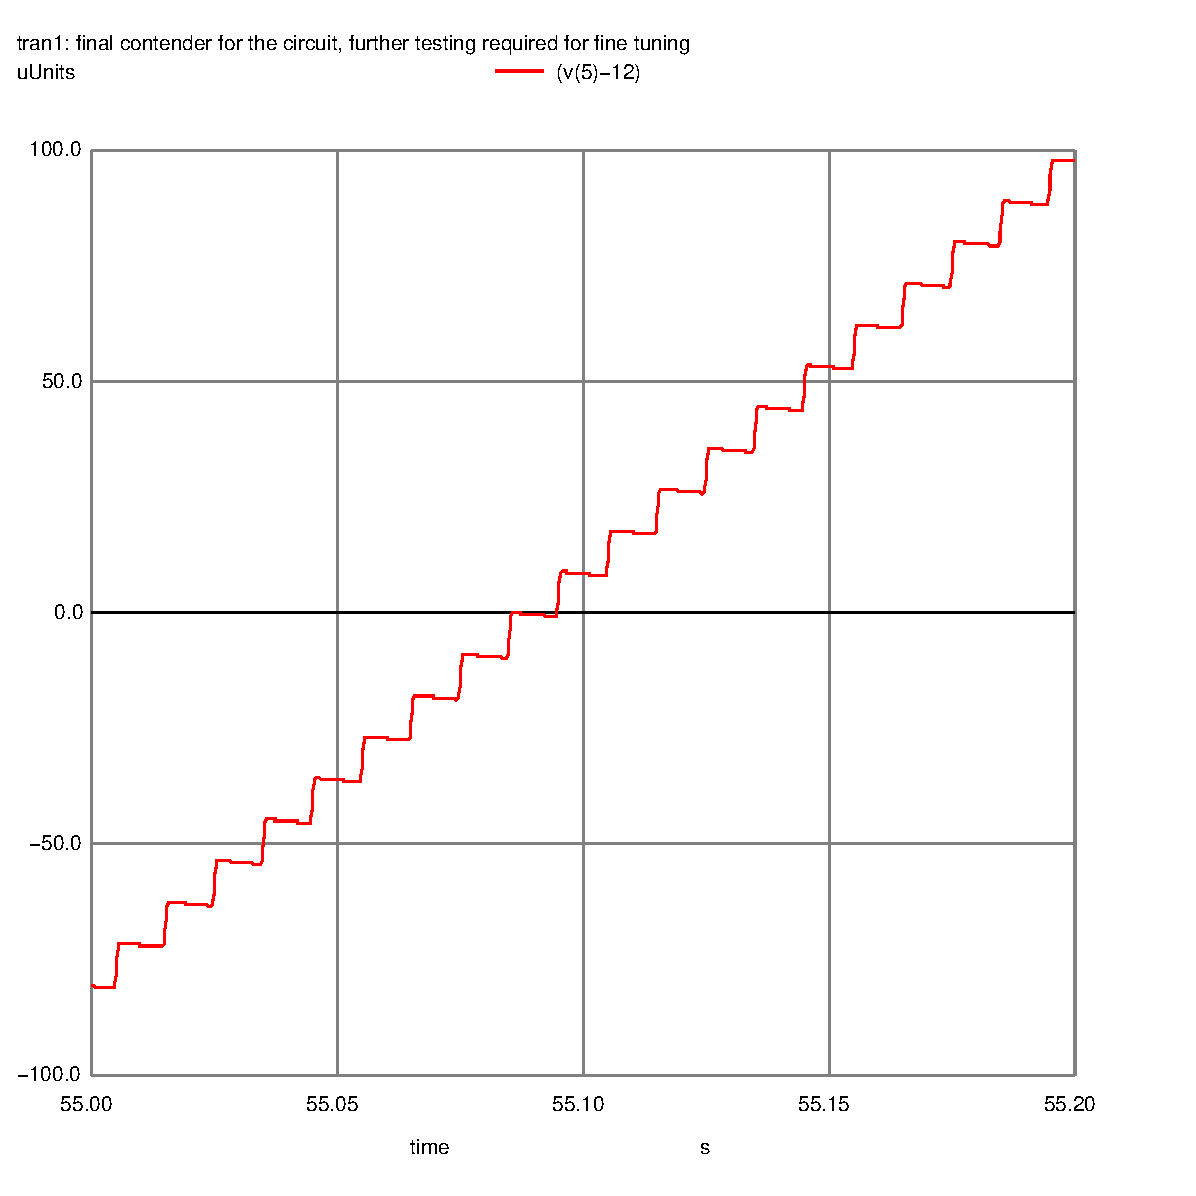
\includegraphics[width=\linewidth]{zoom.ps}
  \caption{No idea what this plot means. Precisa legenda}
  \label{fig:theoplots}
\end{figure}
\FloatBarrier

And finally to conclute the requirements for the simulation analysis, we have computed the results of the voltage ripple and the output DC level. 

%colocar valores
% não consigo encontrar os valores certos para colocar aqui, nomeadamente os do ripple e do DC level, helppp
